\chapter{Experiments and Results}\label{ch:results}

The results are given in the order of the research questions: how the prices behave (RQ1), whether any forecast beats \naive{} (RQ2), and whether the alerts catch sustained rises, and which rule does so best (RQ3, RQ4). Results for 2024 are validation results, on which every setting was chosen. Results for 2025-26 are \emph{retrospective}: no setting was chosen on them, but that period had been looked at in an earlier run of this project.

\section{Experimental Setup}

\subsection{Hardware and software}
\begin{table}[H]\centering\small
\caption[Hardware]{Hardware used.}\label{tab:hardware}
\fittab{\begin{tabular}{lp{9cm}}
\toprule
\textbf{Component} & \textbf{Details} \\
\midrule
Work computer & Windows 10; data conversion and audit, code, local runs while Google Drive could not be mounted in Colab \\
Runs of record & Google Colab, CPU runtime, no GPU \\
Storage & Google Drive folder for data and outputs; public GitHub repository for code and summary tables (no prices) \\
\bottomrule
\end{tabular}
}
\end{table}

\begin{table}[H]\centering\small
\caption[Software]{Software used.}\label{tab:software}
\fittab{\begin{tabular}{lp{8.5cm}}
\toprule
\textbf{Tool} & \textbf{Use} \\
\midrule
Python (Colab) & all notebooks \\
pandas, NumPy & data table, features, scoring \\
LightGBM ($\geq$ 4.3) \cite{lightgbm} & machine-learning forecast \\
statsforecast ($\geq$ 2.0) \cite{statsforecast} & ETS forecast (AutoETS) \\
Matplotlib & figures \\
Gradio 5 \cite{gradio} & monitoring app \\
Git, GitHub & code versions; settings committed before scoring \\
\bottomrule
\end{tabular}
}
\end{table}

\subsection{Implementation details}
The system is written in Python as a small package, \texttt{foodwatch}, that the notebooks call; each notebook does one task (Table~\ref{tab:modules}). The notebooks are generated from one script so that their setup cells are identical: they mount Google Drive, clone the code from the \texttt{main} branch of GitHub, and set the data folder. Settings are read from \path{config/settings.yaml}, and each notebook ends by printing a summary with its checks, so that a run can be confirmed from its last cell.

\begin{table}[H]\centering\small
\caption[Code modules and notebooks]{Code modules and notebooks.}\label{tab:modules}
\begin{tabularx}{\linewidth}{>{\raggedright\arraybackslash}p{4.3cm}X}
\toprule
\textbf{File} & \textbf{Role} \\
\midrule
\texttt{paths.py}, \texttt{load.py} & data folder, settings, readers for the four raw files, hashing \\
\texttt{panel.py}, \texttt{features.py}, \texttt{checks.py} & item $\times$ report-day rows, drivers joined on availability date, data checks \\
\texttt{behaviour.py} & price-change measures and sustained rise episodes \\
\texttt{forecast.py}, \texttt{metrics.py} & naive, ETS and LightGBM on an expanding window; MAE, relative MAE, Diebold--Mariano with Holm \\
\texttt{alerts.py} & ranges from known errors, the three rules, persistence, matching, random-date control, Kupiec test \\
\texttt{monitor.py}, \texttt{app/monitor\_app.py} & day-by-day monitor table and the Gradio app \\
\texttt{report.py} & report tables, figures and the results register \\
notebooks 01--07 & intake, processing, price behaviour, forecast choice and test, alert choice and scoring, report tables, monitor \\
\texttt{tools/} & notebook generator; TCB conversion and audit scripts; thesis files with prices for Overleaf \\
\bottomrule
\end{tabularx}
\end{table}

\subsection{Runs}
Notebooks 01 to 06 were first run on the work computer, while Google Drive could not be mounted in Colab, and then again in Google Colab once it could. Every output file of the Colab runs was byte-identical to the local run (same sha256 hashes); the Colab runs are the runs of record. Each run, its code commit and its file hashes are logged in \path{reports/RUN_LOG.md}.

\section{Dataset}
The data table has 11,296 rows: 8 items on 1,412 report days from 17 May 2021 to 24 October 2026. Prices are missing on 0 to 0.28\,\% of report days per item (Table~\ref{tab:items}). The 2022 gap holds 24 report days. The audit of the converted TCB sheets found no mismatch in 3,060 price cells. Table~\ref{tab:periods} shows how the data is divided in time.

\begin{table}[H]\centering\small
\caption[Distribution of the data over the periods]{Distribution of the data over the periods. Forecasts are per model and horizon; rises are sustained 10\,\% rises by onset date.}\label{tab:periods}
\begin{adjustbox}{max width=\linewidth}\begin{tabular}{lrrrrr}
\toprule
\textbf{Period} & \textbf{Report days} & \textbf{Item-days} & \textbf{Origins} & \textbf{Forecasts} & \textbf{Rises} \\
\midrule
History (May 2021 -- 2023), training only & 480 & 3,840 & -- & -- & 36 \\
2024 validation & 329 & 2,632 & 43 & 344 & 11 \\
2025 -- Oct 2026 test \retro & 603 & 4,824 & 82 & 656 & 23 \\
\midrule
All & 1,412 & 11,296 & 125 & 1,000 & 70 \\
\bottomrule
\end{tabular}\end{adjustbox}
\end{table}


\section{Price Behaviour (RQ1)}\label{sec:res-behaviour}

\subsection{Prices rarely change}
On most report days an item's price is the same as on the previous report day: from 62\,\% of days for broiler chicken to 87\,\% for sugar. Over the whole period the price changed on 12.6\,\% (sugar) to 37.5\,\% (chicken) of report days, and less often in 2024-26 than before (Table~\ref{tab:behaviour}, Figure~\ref{fig:f1}). When a price does change, the typical change is small for the administered items (about 1\,\% for the two oils) and larger for perishables (5\,\% for onion, 6.25\,\% for potato). A price can stay unchanged for long stretches: up to 104 report days for sugar and 102 for palm oil.

\begin{table}[H]\centering\small
\caption[How often and how much prices change]{How often and how much prices change. Change sizes are on days the price changed; unchanged runs are in report days; the last column counts sustained 10\,\% rises in 2021-26.}\label{tab:behaviour}
\fittab{\begin{tabular}{lrrrrrrr}
\toprule
 & \multicolumn{2}{c}{\textbf{Days changed (\%)}} & \multicolumn{2}{c}{\textbf{Change size (\%)}} & \multicolumn{2}{c}{\textbf{Unchanged run}} & \textbf{10\,\%} \\
\cmidrule(lr){2-3}\cmidrule(lr){4-5}\cmidrule(lr){6-7}
\textbf{Item} & 2021-26 & 2024-26 & median & p95 & median & longest & \textbf{rises} \\
\midrule
Chicken - Broiler & 37.5 & 32.4 & 2.70 & 7.58 & 2 & 40 & 8 \\
Egg - Farm & 22.9 & 17.5 & 2.35 & 6.90 & 3 & 44 & 8 \\
Garlic - Imported & 23.6 & 17.7 & 4.00 & 12.91 & 3 & 40 & 12 \\
Onion - Local & 31.8 & 27.0 & 5.00 & 16.72 & 2 & 32 & 19 \\
Palm Oil - Loose & 18.8 & 14.2 & 1.02 & 3.74 & 3 & 102 & 1 \\
Potato & 21.8 & 17.4 & 6.25 & 18.18 & 3 & 75 & 18 \\
Soybean Oil - Loose & 19.4 & 16.6 & 0.88 & 3.01 & 3 & 50 & 1 \\
Sugar & 12.6 & 9.0 & 1.85 & 4.76 & 4 & 104 & 3 \\
\bottomrule
\end{tabular}
}
\source{\path{reports/tables/report/R2_behaviour.csv} (notebook 03).}
\end{table}

\begin{figure}[H]
\centering
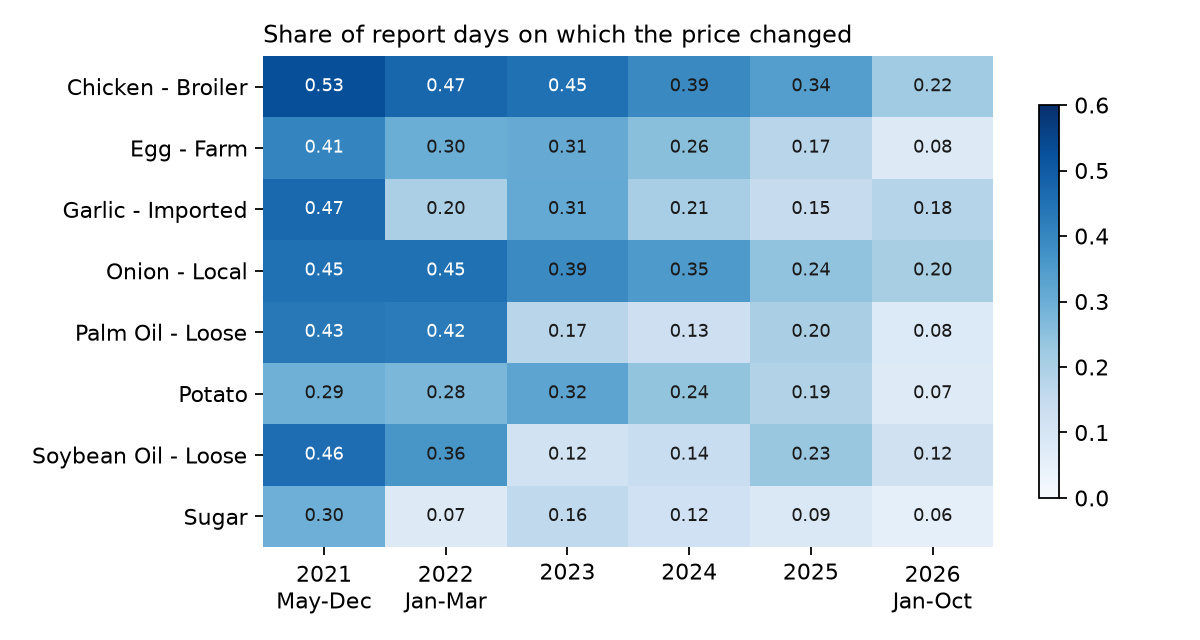
\includegraphics[width=0.9\linewidth]{F1_change_frequency.png}
\caption[Share of report days on which the price changed]{Share of report days on which the price changed, by item and year (2022 covers January to March only, before the gap).}
\label{fig:f1}
\source{\path{reports/figures/F1_change_frequency.png} (notebook 03).}
\end{figure}

This stickiness matters for everything that follows. If the price is unchanged on two days out of three, then ``no change'' is the exact answer on two days out of three, and any model that predicts small movements adds error on those days. The same pattern of infrequent price changes is well documented in studies of retail prices \cite{klenow2010,nakamura2008,cavallo2018}.

\begin{figure}[H]
\centering
\optfig{F2_prices_with_rises.png}{0.95\linewidth}
\caption[Prices of the eight items with sustained rises]{Prices of the eight items with the sustained 10\,\% rises shaded. (This figure shows TCB prices and is kept out of the public repository.)}
\label{fig:f2}
\source{notebook 03, Drive \path{reports/figures/}.}
\end{figure}

\subsection{Sustained rises}
Using the rule of Section~\ref{sec:rise}, the eight items had 70 sustained 10\,\% rises in 2021-26: 11 with onset in 2024 and 23 in 2025-26 (Table~\ref{tab:episodes}). Most of them are in onion (19), potato (18) and imported garlic (12). Palm oil, soybean oil and sugar had no sustained rise in 2024-26, so alerts on these three items cannot be judged as caught or missed; their alerts can only count as unmatched.

\begin{table}[H]\centering\small
\caption[Sustained rise episodes]{Sustained rise episodes by period (onset date), with the 7\,\% and 15\,\% thresholds as a sensitivity check.}\label{tab:episodes}
\fittab{\begin{tabular}{lrrrl}
\toprule
\textbf{Period} & \textbf{7\,\%} & \textbf{10\,\% (main)} & \textbf{15\,\%} & \textbf{Items with no 10\,\% rise} \\
\midrule
2021-26, all & -- & 70 & -- & \\
2024 validation & 17 & 11 & 8 & palm oil, soybean oil, sugar \\
2025-26 \retro & 26 & 23 & 15 & palm oil, soybean oil, sugar \\
\bottomrule
\end{tabular}
}
\source{\path{reports/tables/B5_rise_episodes_by_item_year.csv} (notebook 03).}
\end{table}

\subsection{Before Ramadan}
Table~\ref{tab:ramadan} compares the 30 days before each of the five Ramadans in the data with all other days. Broiler chicken had a positive median change before Ramadan (2.94\,\%) and more rise days (16.1\,\% against 11.1\,\%). Onion and potato had fewer rise days before Ramadan than on other days. The comparison is descriptive: a seasonal pattern is associated with the period and says nothing about why.

\begin{table}[H]\centering\small
\caption[Changes before Ramadan]{Price changes in the 30 days before Ramadan against other days (five Ramadans, about 112 report days per item).}\label{tab:ramadan}
\fittab{\begin{tabular}{lrrrr}
\toprule
 & \multicolumn{2}{c}{\textbf{Median change (\%)}} & \multicolumn{2}{c}{\textbf{Rise days (\%)}} \\
\cmidrule(lr){2-3}\cmidrule(lr){4-5}
\textbf{Item} & before Ramadan & other days & before Ramadan & other days \\
\midrule
Chicken - Broiler & 2.94 & 0 & 16.1 & 11.1 \\
Egg - Farm & $-2.47$ & 0 & 0.0 & 7.3 \\
Garlic - Imported & 0.00 & 0 & 2.7 & 12.7 \\
Onion - Local & $-4.55$ & 0 & 17.9 & 25.2 \\
Palm Oil - Loose & 0.00 & 0 & 3.6 & 0.4 \\
Potato & $-9.76$ & 0 & 8.9 & 24.5 \\
Soybean Oil - Loose & 0.00 & 0 & 0.9 & 0.6 \\
Sugar & 0.00 & 0 & 0.0 & 2.4 \\
\bottomrule
\end{tabular}
}
\source{\path{reports/tables/report/R3_ramadan.csv} (notebook 03).}
\end{table}

\section{Forecast Benchmark (RQ2)}\label{sec:res-forecast}

\subsection{Choice on 2024}
All 16 LightGBM configurations were worse than \naive{} on 2024 (relative MAE 1.047 to 1.536). The simplest one, price history only with 7 leaves, learning rate 0.03 and absolute-error loss, scored best at 1.047 (Table~\ref{tab:grid}). Adding the calendar, weather and exchange-rate drivers made the model worse: the best configuration with drivers scored 1.119. On daily data, these drivers carried no usable signal beyond the recent price path.

\begin{table}[H]\centering\small
\caption[LightGBM configurations on 2024]{LightGBM configurations on 2024 (eight of the sixteen shown, including the best of each feature set; the full grid is in \texttt{M1\_validation\_grid.csv}). Relative MAE is the geometric mean over items of MAE / MAE of \naive{}; above 1 is worse than \naive{}.}\label{tab:grid}
\fittab{\begin{tabular}{llrrrrr}
\toprule
 & & \multicolumn{4}{c}{\textbf{Relative MAE by horizon}} & \\
\cmidrule(lr){3-6}
\textbf{Feature set} & \textbf{Leaves, rate, loss} & 1 & 7 & 14 & 30 & \textbf{All} \\
\midrule
price only & 7, 0.03, l1 (chosen) & 1.114 & 1.029 & 1.035 & 1.014 & \textbf{1.047} \\
price only & 7, 0.05, l1 & 1.219 & 1.033 & 1.062 & 1.040 & 1.086 \\
price only & 31, 0.03, l1 & 1.316 & 1.093 & 1.094 & 1.055 & 1.135 \\
price only & 7, 0.03, huber & 2.098 & 1.134 & 1.072 & 1.001 & 1.264 \\
price + drivers & 7, 0.03, l1 & 1.358 & 1.083 & 1.059 & 1.005 & 1.119 \\
price + drivers & 7, 0.05, l1 & 1.456 & 1.089 & 1.065 & 1.022 & 1.146 \\
price + drivers & 31, 0.03, l1 & 1.617 & 1.165 & 1.145 & 1.080 & 1.236 \\
price + drivers & 7, 0.03, huber & 2.596 & 1.186 & 1.096 & 1.015 & 1.360 \\
\bottomrule
\end{tabular}
}
\source{\path{reports/tables/M1_validation_grid.csv} (notebook 04a, setting committed in \texttt{8d7c145}).}
\end{table}

\subsection{No model beats \naive{}}
Table~\ref{tab:forecast} and Figure~\ref{fig:f3} give the result. Neither ETS nor LightGBM has a relative MAE below 1 at any horizon, in 2024 (1.00 to 1.11) or in 2025-26 (1.01 to 1.21). The gap is largest one day ahead, where \naive{} is right on most days. Where the Diebold--Mariano test finds a significant difference after the Holm correction (3 of 8 comparisons in 2024 and 6 of 8 in 2025-26), the difference is in favour of \naive{}.

The accuracy column shows why accuracy alone would mislead. LightGBM is 99.4\,\% accurate one day ahead in 2025-26, which sounds good, but \naive{} is 99.5\,\% accurate on the same days.

\begin{table}[H]\centering\small
\caption[Forecast benchmark]{Forecast benchmark: MAE of the log change at horizon $h$ (report days), next to \naive{}; relative MAE is the geometric mean over items; Holm $p$ is the corrected Diebold--Mariano $p$-value (``--'': the loss difference has no variance to test).}\label{tab:forecast}
\fittab{\begin{tabular}{llrrrrrr}
\toprule
\textbf{Period} & \textbf{Model} & \textbf{$h$} & \textbf{MAE} & \textbf{MAE naive} & \textbf{Rel.\ MAE} & \textbf{Accuracy} & \textbf{Holm $p$} \\
\midrule
2024 validation & ETS & 1 & 0.009 & 0.009 & 1.060 & 0.991 & 0.003 \\
 & ETS & 7 & 0.032 & 0.032 & 1.010 & 0.968 & 0.027 \\
 & ETS & 14 & 0.051 & 0.051 & 1.004 & 0.948 & 0.146 \\
 & ETS & 30 & 0.083 & 0.083 & 1.002 & 0.914 & 0.281 \\
 & LightGBM & 1 & 0.009 & 0.009 & 1.114 & 0.991 & 0.002 \\
 & LightGBM & 7 & 0.032 & 0.032 & 1.029 & 0.967 & 0.411 \\
 & LightGBM & 14 & 0.052 & 0.051 & 1.035 & 0.947 & 0.434 \\
 & LightGBM & 30 & 0.082 & 0.083 & 1.014 & 0.913 & -- \\
\midrule
2025-26 \retro & ETS & 1 & 0.006 & 0.005 & 1.127 & 0.994 & $<$0.001 \\
 & ETS & 7 & 0.026 & 0.025 & 1.028 & 0.974 & 0.042 \\
 & ETS & 14 & 0.042 & 0.041 & 1.019 & 0.958 & 0.079 \\
 & ETS & 30 & 0.065 & 0.063 & 1.020 & 0.933 & 0.001 \\
 & LightGBM & 1 & 0.006 & 0.005 & 1.213 & 0.994 & $<$0.001 \\
 & LightGBM & 7 & 0.026 & 0.025 & 1.033 & 0.973 & $<$0.001 \\
 & LightGBM & 14 & 0.042 & 0.041 & 1.014 & 0.958 & 0.042 \\
 & LightGBM & 30 & 0.065 & 0.063 & 1.022 & 0.932 & 0.275 \\
\bottomrule
\end{tabular}
}
\source{\path{reports/tables/report/R4_forecast.csv} (notebooks 04a, 04b).}
\end{table}

\begin{figure}[H]
\centering
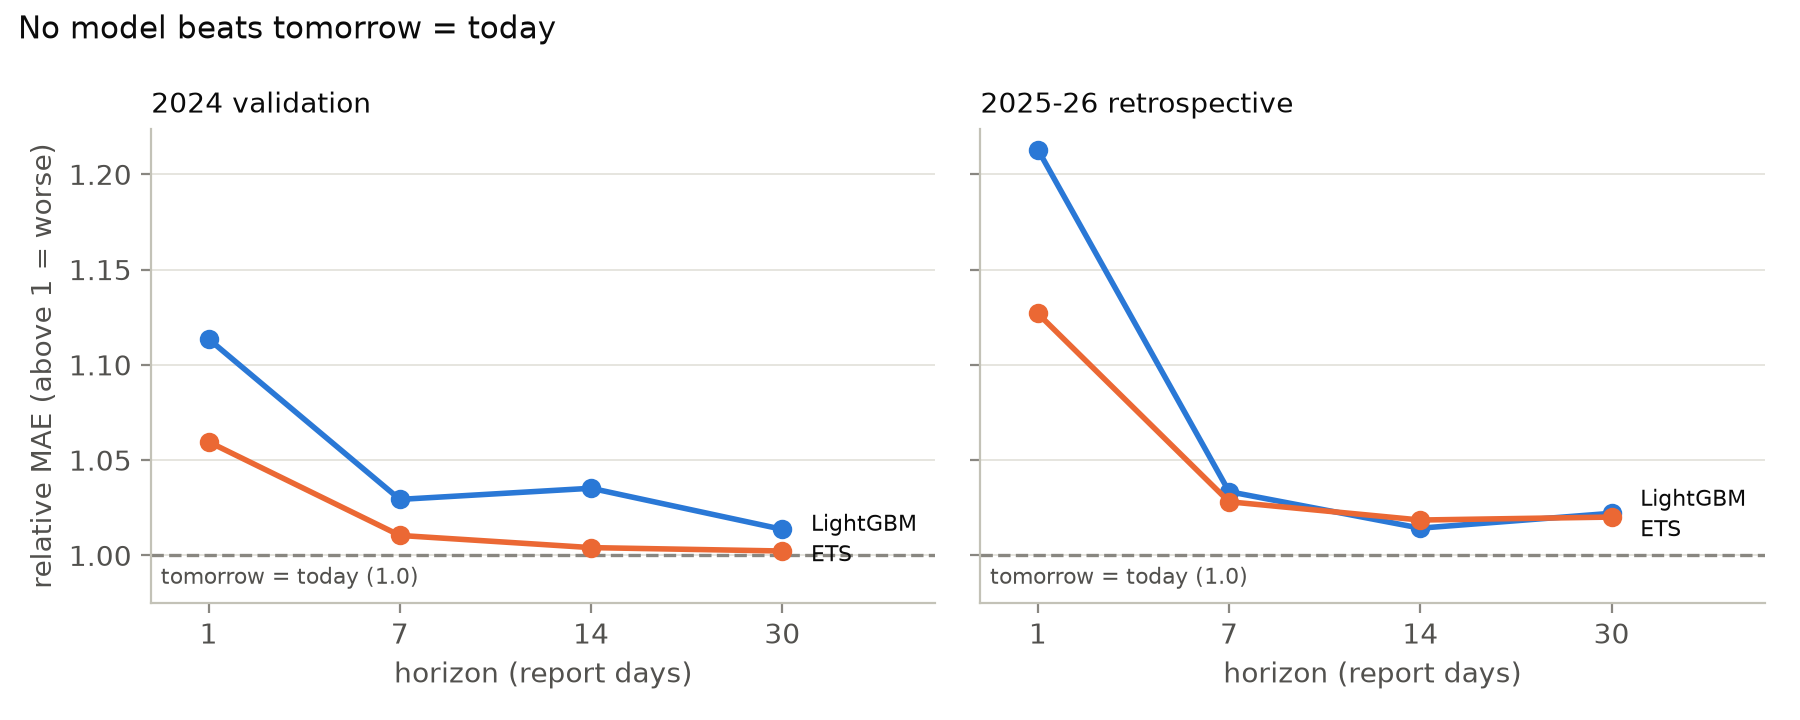
\includegraphics[width=0.85\linewidth]{F3_forecast_vs_naive.png}
\caption[Forecast error relative to \naive{}]{Relative MAE of ETS and LightGBM by horizon; the line at 1 is \naive{}. Every point lies at or above it.}
\label{fig:f3}
\source{\path{reports/figures/F3_forecast_vs_naive.png} (notebook 06).}
\end{figure}

\section{Alert Rules (RQ3, RQ4)}\label{sec:res-alerts}

\subsection{Settings chosen on 2024}
Table~\ref{tab:alertchoice} lists every candidate on 2024. For the ML range (A) and the simple range (B), the 0.90 level gave more than 2 unmatched alert runs per item-year, so the 0.95 level was chosen. For the fixed rise (C), 7\,\% was the most sensitive threshold within the target. These three settings were committed in \texttt{e0cfa06} before any rule was scored on 2025-26.

\begin{table}[H]\centering\small
\caption[Alert settings on 2024]{Alert settings on 2024 (11 sustained rises, 10.53 item-years). The chosen setting is the most sensitive one with at most 2 unmatched alert runs per item-year.}\label{tab:alertchoice}
\fittab{\begin{tabular}{llrrrrl}
\toprule
\textbf{Rule} & \textbf{Setting} & \textbf{Caught} & \textbf{Runs} & \textbf{Precision} & \textbf{Unmatched / item-year} & \textbf{Chosen} \\
\midrule
A. ML range & 0.90 & 9/11 & 39 & 0.23 & 2.85 & \\
 & 0.95 & 6/11 & 17 & 0.35 & 1.04 & yes \\
 & 0.975 & 5/11 & 13 & 0.38 & 0.76 & \\
 & 0.99 & 4/11 & 10 & 0.40 & 0.57 & \\
\midrule
B. Simple range & 0.90 & 9/11 & 36 & 0.25 & 2.56 & \\
 & 0.95 & 8/11 & 20 & 0.40 & 1.14 & yes \\
 & 0.975 & 5/11 & 14 & 0.36 & 0.85 & \\
 & 0.99 & 4/11 & 11 & 0.36 & 0.66 & \\
\midrule
C. Fixed rise & 3\,\% & 10/11 & 58 & 0.17 & 4.56 & \\
 & 5\,\% & 10/11 & 39 & 0.26 & 2.75 & \\
 & 7\,\% & 10/11 & 27 & 0.37 & 1.61 & yes \\
 & 10\,\% & 9/11 & 15 & 0.60 & 0.57 & \\
\bottomrule
\end{tabular}
}
\source{\path{reports/tables/A1_alert_choice.csv} (notebook 05a, committed in \texttt{e0cfa06}).}
\end{table}

\subsection{All three rules beat random dates}
Table~\ref{tab:alertrules} and Figure~\ref{fig:f4} give the scores. In 2024 the ML range caught 6 of 11 sustained rises, the simple range 8 and the fixed rise 10. In 2025-26 \retro{} the ML range caught 17 of 23, the simple range 15 and the fixed rise 22. The same number of alert runs placed on random dates caught far fewer: for the two ranges, the real recall was 2.5 to 2.8 times the random-date recall. In none of the 300 random draws did the random recall reach the real one, for any rule in either period ($p = 0.003$, the smallest value the test can give).

Alerts start a median of 1.5 to 2 report days after a rise begins for the two ranges. This is detection of a rise that is under way, not early warning.

About 6 of every 10 alert runs of the two ranges do not match a sustained 10\,\% rise (precision 0.35 to 0.40). That is roughly 1.0 to 1.3 unmatched runs per item per year. An alert means that the price is unusually high for that item; not every unusual rise goes on to last long enough to count as a sustained 10\,\% rise.

\begin{table}[H]\centering\small
\caption[Alert rules scored against sustained rises]{Alert rules scored against sustained 10\,\% rises. Random = mean recall of the same alert runs on random dates (300 draws); $p$ = random-date $p$-value; Runs = alert runs; Delay = median report days from onset to the matched alert.}\label{tab:alertrules}
\fittab{\begin{tabular}{llrrrrrrr}
\toprule
\textbf{Period} & \textbf{Rule} & \textbf{Caught} & \textbf{Recall} & \textbf{Random} & \textbf{$p$} & \textbf{Runs} & \textbf{Precision} & \textbf{Delay} \\
\midrule
2024 validation & A. ML range & 6/11 & 0.55 & 0.20 & 0.003 & 17 & 0.35 & 1.5 \\
 & B. Simple range & 8/11 & 0.73 & 0.30 & 0.003 & 20 & 0.40 & 2 \\
 & C. Fixed 7\,\% & 10/11 & 0.91 & 0.49 & 0.003 & 27 & 0.37 & 0.5 \\
\midrule
2025-26 \retro & A. ML range & 17/23 & 0.74 & 0.28 & 0.003 & 42 & 0.40 & 2 \\
 & B. Simple range & 15/23 & 0.65 & 0.25 & 0.003 & 39 & 0.38 & 2 \\
 & C. Fixed 7\,\% & 22/23 & 0.96 & 0.31 & 0.003 & 30 & 0.73 & 2 \\
\bottomrule
\end{tabular}
}
\source{\path{reports/tables/report/R5_alert_rules.csv} (notebook 05b).}
\end{table}

\begin{figure}[H]
\centering
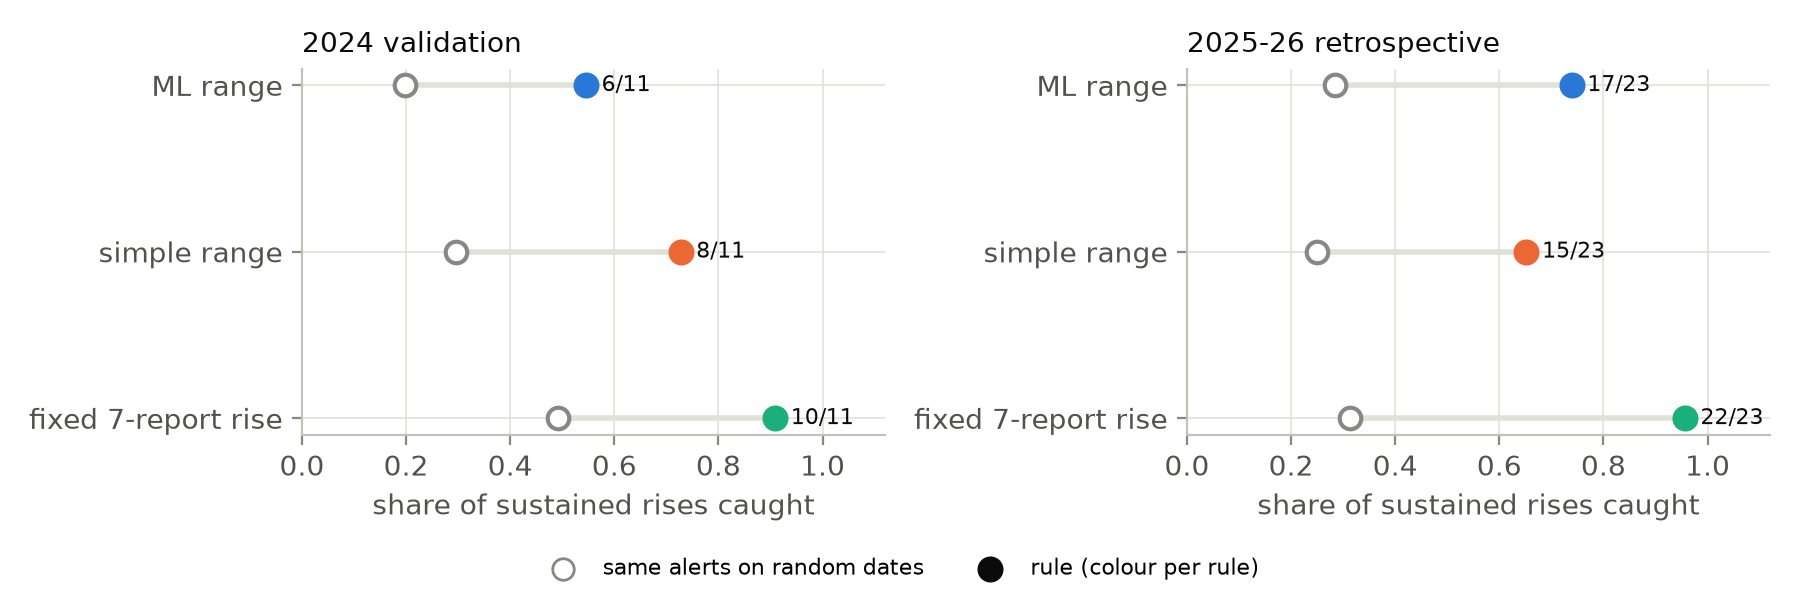
\includegraphics[width=0.85\linewidth]{F4_alert_recall.png}
\caption[Sustained rises caught, against random dates]{Share of sustained rises caught by each rule, against the same alert runs on random dates.}
\label{fig:f4}
\source{\path{reports/figures/F4_alert_recall.png} (notebook 06).}
\end{figure}

\subsection{The ML range adds nothing over the simple range}
The ML range and the simple range catch almost the same rises (Table~\ref{tab:overlap}). In 2024 the simple range caught two rises that the ML range missed and the reverse never happened; in 2025-26 the ML range caught two that the simple range missed and the reverse never happened. Over the two periods each range caught two rises the other missed. This is what Section~\ref{sec:res-forecast} leads one to expect: since the LightGBM forecast is close to \naive{}, the two ranges are close too. For a monitor, the simple range is enough: it catches the same rises and needs no model to be trained or maintained.

\begin{table}[H]\centering\small
\caption[Rises caught by the ML range and the simple range]{Sustained rises caught by the ML range and the simple range.}\label{tab:overlap}
\fittab{\begin{tabular}{lrrrrr}
\toprule
\textbf{Period} & \textbf{Rises} & \textbf{Both} & \textbf{ML range only} & \textbf{Simple range only} & \textbf{Neither} \\
\midrule
2024 validation & 11 & 6 & 0 & 2 & 3 \\
2025-26 \retro & 23 & 15 & 2 & 0 & 6 \\
\bottomrule
\end{tabular}
}
\source{\path{reports/tables/report/R5b_rule_overlap.csv} (notebook 05b).}
\end{table}

\subsection{The fixed rise is a reference, not the winner}
Rule C catches the most rises (10 of 11 and 22 of 23), and in 2025-26 it also has the highest precision. This should not be read as a win. A rise of 7\,\% over 7 report days is very close to the definition of the thing being scored, a rise of 10\,\% over 14 report days lasting 5 days, so its score is partly built in. It also uses one threshold for every item, so it cannot tell an ordinary move of a volatile item such as onion from an unusual move of a stable one. It is reported as a reference point for the two ranges.

\subsection{Results by item}
Table~\ref{tab:byitem} shows each item. Onion, potato and garlic hold most of the rises. On the three items without any sustained rise, the ranges still raised 2 to 5 alert runs per period; these are the unmatched alerts of a sticky price that moved by more than usual.

\begin{table}[H]\centering\small
\caption[Alerts by item]{Rises caught / rises (alert runs) by item and rule. ``--'': no sustained rise in the period, so the alerts cannot be judged.}\label{tab:byitem}
\fittab{\begin{tabular}{lllllll}
\toprule
 & \multicolumn{3}{c}{\textbf{2024 validation}} & \multicolumn{3}{c}{\textbf{2025-26 \retro}} \\
\cmidrule(lr){2-4}\cmidrule(lr){5-7}
\textbf{Item} & A & B & C & A & B & C \\
\midrule
Chicken - Broiler & 1/1 (3) & 1/1 (4) & 1/1 (5) & 1/3 (4) & 1/3 (4) & 2/3 (3) \\
Egg - Farm & 1/1 (1) & 1/1 (1) & 1/1 (3) & 3/3 (7) & 3/3 (6) & 3/3 (4) \\
Garlic - Imported & 1/2 (1) & 1/2 (1) & 1/2 (1) & 4/4 (7) & 4/4 (8) & 4/4 (7) \\
Onion - Local & 2/4 (2) & 3/4 (3) & 4/4 (10) & 5/7 (6) & 5/7 (6) & 7/7 (9) \\
Potato & 1/3 (2) & 2/3 (3) & 3/3 (8) & 4/6 (5) & 2/6 (3) & 6/6 (6) \\
Palm Oil - Loose & -- (3) & -- (3) & -- (0) & -- (4) & -- (4) & -- (0) \\
Soybean Oil - Loose & -- (3) & -- (3) & -- (0) & -- (4) & -- (3) & -- (0) \\
Sugar & -- (2) & -- (2) & -- (0) & -- (5) & -- (5) & -- (1) \\
\bottomrule
\end{tabular}
}
\source{\path{reports/tables/report/R6_focus_items.csv} (notebook 05b).}
\end{table}

\subsection{Range coverage}
A 95\,\% upper bound should hold the price on about 95\,\% of days. In 2024 it did: 94.5\,\% for the ML range and 94.6\,\% for the simple range, consistent with 95\,\% by Kupiec's test (Table~\ref{tab:coverage}). In 2025-26 coverage was 93.4\,\% and 93.9\,\%, slightly but significantly below 95\,\%. A range built from the last 120 errors adapts slowly when prices become more volatile.

\begin{table}[H]\centering\small
\caption[Coverage of the expected range]{Share of days at or below the upper bound, against the nominal 95\,\%, with Kupiec's test.}\label{tab:coverage}
\fittab{\begin{tabular}{llrrrr}
\toprule
\textbf{Period} & \textbf{Rule} & \textbf{Days} & \textbf{Nominal} & \textbf{Coverage} & \textbf{Kupiec $p$} \\
\midrule
2024 validation & A. ML range & 2632 & 0.95 & 0.945 & 0.205 \\
 & B. Simple range & 2632 & 0.95 & 0.946 & 0.358 \\
2025-26 \retro & A. ML range & 4824 & 0.95 & 0.934 & $<$0.001 \\
 & B. Simple range & 4824 & 0.95 & 0.939 & 0.001 \\
\bottomrule
\end{tabular}
}
\source{\path{reports/tables/report/R7_range_coverage.csv} (notebook 05b).}
\end{table}

\section{Sample Input and Output}\label{sec:res-monitor}
This section follows one real case through the system, in the order in which the system processes it: the sustained rise of local onion that began on 2 November 2025 (2025-26, retrospective). The rise lasted 16 report days, to 17 November 2025, with a peak rise of 57\,\% over 14 report days.

\subsection{Input}
The input on each report day is the TCB row of the item, joined with its drivers (Table~\ref{tab:datasample}), and the 7-day forecast made one week earlier. For onion, the drivers are the weather columns; the chosen LightGBM uses price history only.

\subsection{Expected range}
On each day $t$, the upper bound of the ML range is the LightGBM forecast made at $t-7$ plus the 95th percentile of onion's last 120 forecast errors known at $t-7$. The bound is fixed before day $t$ is seen.

\subsection{Alert decision}
Table~\ref{tab:worked} follows the days around the onset. Onion was above the bound on the onset day and the next day, which is not yet an alert. On 4 November 2025, the third day above the bound in the last five, the alert run started: 2 report days after the onset.

\begin{table}[H]\centering\footnotesize
\caption[Worked example: onion, November 2025]{Worked example: local onion around the onset of the rise of 2 November 2025, under the ML range (prices in Tk; change over 7 report days).}\label{tab:worked}
\opttab{worked_example}
\source{\texttt{processed/monitor\_8.csv} on Drive (contains prices; not in the public repository).}
\end{table}

\subsection{Output in the app}
Figures~\ref{fig:app-status} to \ref{fig:app-how} show the four tabs of the app for this case.

\begin{figure}[H]
\centering
\optfig[245 30 245 0]{monitor_status.png}{\linewidth}
\caption[App: status on a day]{App, ``Status on a day'': all eight items on 4 November 2025 under the ML range; onion is in alert.}
\label{fig:app-status}
\end{figure}

\begin{figure}[H]
\centering
\optfig[240 10 255 0]{monitor_item.png}{\linewidth}
\caption[App: item chart]{App, ``Item'': onion from October to November 2025 with the upper bound, the sustained rise shaded and the start of the alert run.}
\label{fig:app-item}
\end{figure}

\begin{figure}[H]
\centering
\optfig[310 45 310 0]{monitor_log.png}{\linewidth}
\caption[App: alert log]{App, ``Alert log'': alert runs of the ML range in 2025-26 with the hindsight match.}
\label{fig:app-log}
\end{figure}

\begin{figure}[H]
\centering
\optfig{monitor_how.png}{\linewidth}
\caption[App: how it works]{App, ``How it works'': the three rules and their scores.}
\label{fig:app-how}
\end{figure}

\subsection{Validation}
In hindsight, the alert run that started on 4 November 2025 lies inside the match window of the rise (14 report days before the onset to 7 after its end), so it counts as a caught rise in Table~\ref{tab:alertrules}. For the whole period, the app's alert flags were checked to be identical to those scored in notebook 05b, and its counts of alert runs equal Table~\ref{tab:alertrules}. Figure~\ref{fig:f5} shows the alerts of the three rules on onion, potato and egg over 2024-26.

\begin{figure}[H]
\centering
\optfig{F5_prices_with_alerts.png}{0.95\linewidth}
\caption[Prices with alerts for onion, potato and egg]{Onion, potato and egg prices, 2024 to October 2026, with sustained rises shaded and the start of each alert run of the three rules.}
\label{fig:f5}
\source{notebook 06, Drive \path{reports/figures/}.}
\end{figure}


\section{Discussion}

\subsection{Why \naive{} wins}
The forecast result follows from the price behaviour. TCB records a price that is unchanged on 62 to 87\,\% of report days and that moves in steps of at least Tk 0.5. On such a series, the last price is the best guess most of the time. A model that learns average movements from history spreads small predicted changes over many days on which nothing happens, and loses more on those days than it gains on the few days with a large move. This is the same lesson as the long line of studies in which the random walk is hard to beat out of sample \cite{meese1983}, and it matches the Bangladeshi benchmark in which naive persistence won on commodities that behave like a random walk \cite{agripricebd}. The drivers did not help because, on a daily scale, weather and the exchange rate change slowly and are already reflected in the recent price path.

\subsection{What the alerts can and cannot say}
The alerts work: all three rules catch far more sustained rises than the same number of alerts on random dates, and the ranges do so a median of 1.5 to 2 report days after a rise begins. An alert says that the price of an item has stayed above what its own recent behaviour would lead one to expect. Such a rise is \unexpl{} in this system. The alert does not say why the price rose; finding that out needs other evidence.

\subsection{Which rule to use}
The ML range and the simple range catch nearly the same rises, so the machine-learning model adds nothing to the alerts. For a monitor that someone has to keep running, the simple range is the better choice: same rises, no model to train, and a rule that is easy to explain. The app shows the ML range first so that the comparison stays visible, and it states this finding beside it.

\section{Threats to Validity}\label{sec:threats}
\begin{itemize}[leftmargin=*,itemsep=2pt]
\item \textbf{Retrospective test period.} 2025-26 had been looked at by an earlier run of the project. No setting in this run was chosen on it, and the commits show the order, but the design of the comparison was made after those earlier results were known.
\item \textbf{Item choice.} The eight items were chosen after the earlier 54-item results had been seen.
\item \textbf{Few rises.} 2024 has 11 sustained rises and 2025-26 has 23. Rates are always shown with their counts. The random-date test does not need large samples, and both periods point the same way.
\item \textbf{Three items without rises.} For palm oil, soybean oil and sugar, recall cannot be measured.
\item \textbf{Rule C is partly circular}, as discussed above.
\item \textbf{The reference is a definition.} A sustained 10\,\% rise over 14 report days is one reasonable definition among several; the 7\,\% and 15\,\% counts show how much it matters.
\item \textbf{Data.} The audit confirms the copying of the TCB sheets, not the accuracy of what TCB recorded. TCB reports a range for Dhaka markets, and the midpoint is used as the price.
\item \textbf{Coverage} in 2025-26 is slightly below its nominal level.
\end{itemize}
